\documentclass[b,e,cours]{D:/Dropbox/enseignement/CPGE/raphaelpoiree/paquets/classe_kara}
\begin{document}
\newcommand*{\partie}{Modèles}
\newcommand*{\titre}{Modèle de cours}
\newcommand*{\numero}{-1}
\newcommand*{\prerequis}{\item Prérequis}
\newcommand*{\connaissances}{\item connaissance}
\newcommand*{\savoirfaire}{\item savoirfaire}
\newcommand*{\organisation}{\item Organisation}
\newcommand*{\afaire}{\item gérer les références.}


\newpage
%%%%%%%%%%%%%%%%%%%%%%%%%%%% VERSION ARTICLE %%%%%%%%%%%%%%%%%%%%%%%%%%%%%%%%%%%
\ifthenelse{\boolean{Cours}}{

\mode<article>{
\thispagestyle{empty}
\vspace{0.2cm}

\begin{center}

\rule{\linewidth}{5pt}\\
\begin{minipage}{0.1\linewidth}
\begin{center}

\includegraphics[width=\textwidth]{D:/Dropbox/enseignement/CPGE/raphaelpoiree/paquets/logoBaggio.jpg}
\end{center}
\end{minipage}
\begin{minipage}{0.8\linewidth}
\begin{center}
\vspace{0.2cm}

\large{\MakeUppercase{\partie}}\\

\vspace{0.2cm}

\huge{
Cours \numero \ - \titre
}
\end{center}
\end{minipage}
\begin{minipage}{0.1\linewidth}
\end{minipage}

\vspace{0.4cm}
\rule{\linewidth}{5pt}

\end{center}

\begin{center}
\MakeUppercase{\etablissement} - \MakeUppercase{\auteur} - \MakeUppercase{\classe} - \MakeUppercase{\annee}
\end{center}

\tableofcontents
%\minitoc

%\vfill

%\vspace{1cm}
\ifthenelse{\boolean{version_prof}}{

\ifthenelse{\boolean{version_kara}}{
		\begin{bclogo}[couleur = red!70,logo=\bcpanchant]{À faire}
		\begin{itemize}
		\afaire
		\end{itemize}
		\end{bclogo}
		}{} %fin ifthenelse version kara

		\begin{bclogo}[couleur = green!30,logo=\bcoutil]{Pré-requis}
		\begin{itemize}
		\prerequis
		\end{itemize}
		\end{bclogo}
\begin{minipage}{0.5\textwidth}
		\begin{bclogo}[couleur = yellow!30,logo=\bctrombone]{Connaissances}
		\begin{itemize}
		\connaissances
		\end{itemize}
		\end{bclogo}
\end{minipage}
\begin{minipage}{0.5\textwidth}
		\begin{bclogo}[couleur = yellow!30,logo=\bctrombone]{Savoir-faire}
		\begin{itemize}
		\savoirfaire
		\end{itemize}
		\end{bclogo}
\end{minipage}

		\begin{bclogo}[couleur = white!30,logo=\bccalendrier]{Organisation}
		\begin{itemize}
		\organisation
		\end{itemize}
		\end{bclogo}
		}{}
%	 \lhead{\MakeUppercase{\partie}}
%    \chead{Cours \numero}
%    \rhead{\titre}
%    \lfoot{
\includegraphics[width=1.2cm]{paquets/Creative_Commons.png} \hspace{0.1cm} \etablissement - \auteur\\ \ }
%    \cfoot{\thepage/\pageref{LastPage}}
%    \rfoot{Version \version - \classe}
%    \renewcommand{\headrulewidth}{0.2pt}
%    \renewcommand{\footrulewidth}{0.2pt}	
}%% Fin mode article

%%%%%%%%%%%%%%%%%%%%%%%%%  MODE PRÉSENTATION %%%%%%%%%%%%%%%%%%%%%%%%%%%%%%%%%%%

\mode<presentation>{
\title{Cours \numero \ - \titre}
\date{Version \version \  du \today}
\author{\auteur}
\institute{\etablissement -  \classe}

%%%%% PREMIÈRE SLIDE
\begin{frame}

	\begin{center}
		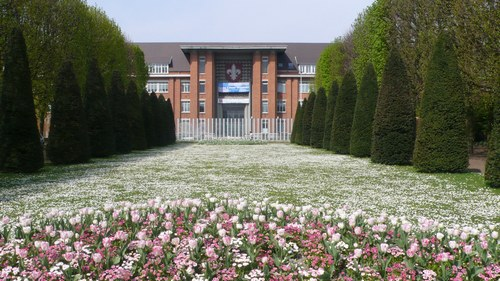
\includegraphics[height=3cm]{img/bandeau_1}
	\end{center}


	\maketitle

\end{frame}



\ifthenelse{\boolean{version_prof}}{
\begin{frame}[allowframebreaks]\titreslide{Informations professeur}
		\ifthenelse{\boolean{version_kara}}{
		\begin{bclogo}[couleur = red!70,logo=\bcpanchant]{À faire}
		\begin{itemize}
		\afaire
		\end{itemize}
		\end{bclogo}}{}

		
		\begin{bclogo}[couleur = white!30,logo=\bccalendrier]{Organisation}
		\begin{itemize}
		\organisation
		\end{itemize}
		\end{bclogo}
\end{frame}}{}
}%% Fin mode présentation
}{}%% Fin version cours

%% Version EXO

\ifthenelse{\boolean{Exo}}{
\title{Exercices}
\mode<article>{
	\lhead{\MakeUppercase{\partie}}
%    \chead{Exercice \numero}
    \rhead{Exercices}
    \lfoot{
\includegraphics[width=1.2cm]{paquets/Creative_Commons.png} \hspace{0.1cm} \etablissement - \auteur }
    \cfoot{\thepage/\pageref{LastPage}}
    \rfoot{Version \version}
    \renewcommand{\headrulewidth}{0.2pt}
    \renewcommand{\footrulewidth}{0.2pt}
    }% Fin mode article	
\mode<presentation>{
\maketitle
}
}{}%% Fin version exercice


\ifthenelse{\boolean{TD}}{
\title{TD \numero}
\mode<article>{
}% Fin mode article	
\mode<presentation>{
\maketitle
}
}{}%% Fin version TD



\section{Introduction}
\begin{frame}\titreslide{Introduction}
Le but de ce modèle \LaTeX de cours/diapo est de générer un document et des diapos, en versions étudiant et professeur à partir du même fichier.
\end{frame}
\begin{frame}\titreslide{Sources}
Les documents et diapos sont réalisés simultanément avec le package beamerarticle.\\
Les boîtes sont basées sur le package de R. ALLAIS~\cite{raphaelallais}.
\end{frame}

\subsection{Comparaison de différentes solutions}
\begin{frame}\titreslide{Comparaison différentes solutions}
\PROF{Faire un beau tableau\\}
\textbf{Document papier seul}~~\\
Le cours est donné aux étudiants. Le prof lit le cours au tableau ou le fait défiler.\\
\textbf{Diapos seules}~~\\
Le cours est l'impression des diapos. Le prof présente les diapos.\\
\textbf{Document papier + Diapos}\\
L'étudiant a un document et le prof fait défiler les diapos.
\end{frame}


\section{Commandes}
\subsection{Différence document/diapos}
\begin{frame}[fragile]\titreslide{Différence document/diapos}
\textbf{Texte qui apparaît que dans le document :}\\
\mode<article>{Je n'apparais que dans le document.}
\textbf{Texte qui apparaît que dans les diapos :}\\
\mode<presentation>{Je n'apparais que dans les diapos.}
\textbf{Texte qui apparaît dans le document et dans les diapos :}\\
J'apparais dans le document et les diapos.

\begin{verbatim}
\textbf{Texte qui apparaît que dans le document :}\\
\mode<article>{Je n'apparais que dans le document.}
\textbf{Texte qui apparaît que dans les diapos :}\\
\mode<presentation>{Je n'apparais que dans les diapos.}
\textbf{Texte qui apparaît dans le document et dans les diapos :}\\
J'apparais dans le document et les diapos.
\end{verbatim}
\end{frame}


\subsection{Différence version professeur/étudiant}

\begin{frame}\titreslide{Différence version professeur/étudiant}
\textbf{Texte qui apparaît dans la version prof et étu :}\\
J'apparais dans la version prof et étudiant.\\

\textbf{Texte qui apparaît que dans la version prof :}\\
\PROF{Texte qui n'apparaît que dans la version prof}
%
%\textbf{Texte qui apparaît que dans la version kara:}\newline
%\KARA{Texte qui n'apparaît que dans la version prof}
\end{frame}

%\subsection{Minipages}
%\begin{frame}\titreslide{Minipages}
%
%
%\end{frame}


\subsection{Texte à trous}

\begin{frame}[fragile]\titreslide{Texte à trous}
Afin de forcer les étudiants de suivre le cours, un moyen pédagogique est l'utilisation de \trouer{trous}. Ces \trouer{trous} n'apparaissent que dans la version prof et sont remplacés par des \trouer{blancs} dans la version étudiants...\\
La commande pour trouer du texte est : \begin{verbatim} \trouer{texte à cacher/afficher} \end{verbatim}


Un trou sur plusieurs lignes :

\begin{itemize}
\item \trouer{Ce texte est troué}
\item \trouer{Ce texte est troué}
\end{itemize}



Ligne après les trous.

\end{frame}

\subsection{Correction}
\begin{frame}[fragile]\titreslide{Correction}

La correction apparaît dans la version prof et apparaît en blanc dans la version étudiants...\newline
\textbf{33 Cr Mo V 12-9 : } \uncover<2>{\correction{acier faiblement allié à 0.33\% de carbone, 3\% de chrome, 0.9\% de molybdène et vanadium < 1\%}}\\
\end{frame}

%\subsection{Texte caché interactif}
%%\begin{frame}\titreslide{Texte caché interactif}
%%\KARA{http://forum.mathematex.net/latex-f6/souligner-un-phantom-en-pointilles-avec-retour-a-la-ligne-t10057.html\newline}
%%Une partie de ce texte est \hide{caché de manière interactive}. Il suffit de cliquer dessus pour \hide{l'afficher}...\\
%%
%%Aller, \hide{on teste le texte caché de manière interactive sur plusieurs lignes pour voir }\newline \hide{s'il est capable de passer à la ligne suivante...}
%%\end{frame}

\subsection{Insertion d'une image}
\begin{frame}\titreslide{Insertion d'une image}
	\begin{figure}[h]
		\begin{center}
			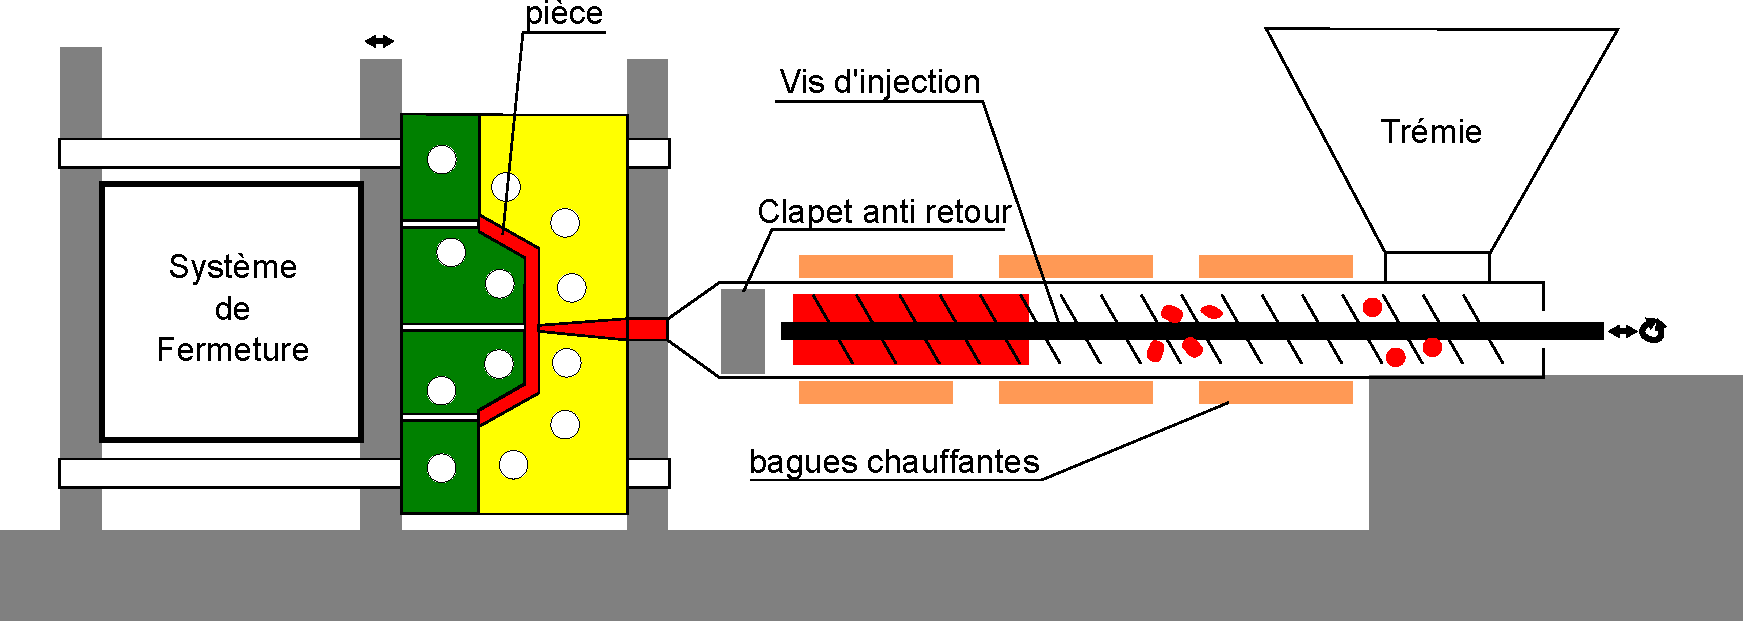
\includegraphics[width=0.8\textwidth]{img/schema_presse_a_injecter.pdf} 
			\caption{Schéma d'une presse à injecter}
			\label{schema_presse_a_injecter}
		\end{center}
	\end{figure}
\end{frame}


%	\begin{figure}[h]
%		\begin{center}
%			\includegraphics[width=0.8\textwidth]{img/nom_image.pdf} 
%			\caption{Légende image}
%			\label{label_image}
%		\end{center}
%	\end{figure}
%
%\mode<presentation>{
%\subsection{Insertion d'une vidéo}
%\begin{frame}\titreslide{Insertion d'une vidéo}
%	\begin{figure}
%		\begin{center}
%			\movie[autostart,showcontrols]{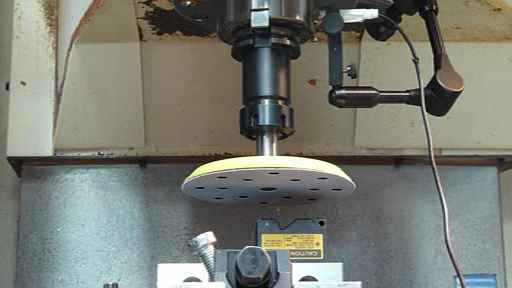
\includegraphics[width=\textwidth]{mov/video_papier_abrasif.png}}{mov/video_papier_abrasif.avi}
%		\end{center}
%	\end{figure}
%\end{frame}
%}
%
%\subsection{Insertion d'une animation flash}
%\begin{frame}\titreslide{Insertion d'une animation flash}
%\begin{figure}
%	\begin{center}
%	\includemedia[
%    width=\textwidth,
%    height=0.8\textheight,
%    addresource=mov/MccComplet.swf,
%    transparent,
%    activate=onclick,
%    deactivate=onclick]{}{mov/MccComplet.swf}
%    \legend{Animation d'un moteur à courant continu}
%    \end{center}
%\end{figure}
%\end{frame}
%
%\begin{frame}\titreslide{Insertion d'une animation flash}
%\begin{figure}
%	\begin{center}
%	\includemedia[
%    width=\textwidth,
%    height=0.8\textheight,
%    addresource=mov/chute.swf,
%    transparent,
%    activate=onclick,
%    deactivate=onclick]{}{mov/chute.swf}
%    \legend{Chute d'un corps dans un champ de pesanteur uniforme}
%    \end{center}
%\end{figure}
%\end{frame}
%
%\begin{frame}\titreslide{Insertion d'une animation flash}
%\begin{figure}
%	\begin{center}
%	\includemedia[
%    width=\textwidth,
%    height=0.8\textheight,
%    addresource=mov/euler.swf,
%    transparent,
%    activate=pageopen,
%    deactivate=onclick]{}{mov/euler.swf}
%    \legend{Les angles d'Euler}
%    \end{center}
%\end{figure}
%\end{frame}
%
%
%\begin{frame}\titreslide{Insertion d'une animation flash}
%\begin{figure}
%	\begin{center}
%	\includemedia[
%    width=\textwidth,
%    height=0.8\textheight,
%    addresource=mov/euler.swf,
%    transparent,
%    activate=pageopen,
%    deactivate=onclick]{}{mov/anim_procedes/procindus.swf}
%    \legend{Procédés industriels}
%    \end{center}
%\end{figure}
%\end{frame}
%
%\begin{frame}\titreslide{Insertion d'une animation flash}
%\includemedia[flashvars={source=http://mp3.live.tv-radio.com/franceculture/all/franceculturehautdebit.mp3
%&autoPlay=true},
%transparent]{\textcolor{blue}{\fbox{Listen live to Radio France Culture}}}{http://mirrors.ibiblio.org/pub/mirrors/CTAN/macros/latex/contrib/media9/players/APlayer.swf}
%
%\end{frame}
%
%\begin{frame}\titreslide{Insertion d'une image3D}
%\includemedia[
%width=0.8\textwidth ,height=0.4\textwidth,
%add3Djscript=asylabels.js, %upright text labels
%add3Djscript=3Dspintool.js, %let scene rotate about z-axis
%% 3Dcoo, 3Droo values found with ‘Generate Default View’ from
%% context menu
%3Dmenu,
%3Dc2c=4 2 3,
%3Dcoo=4.413303375244141 2.195653200149536 -0.000011444091796875,
%3Droo=429.49035778293376,
%]{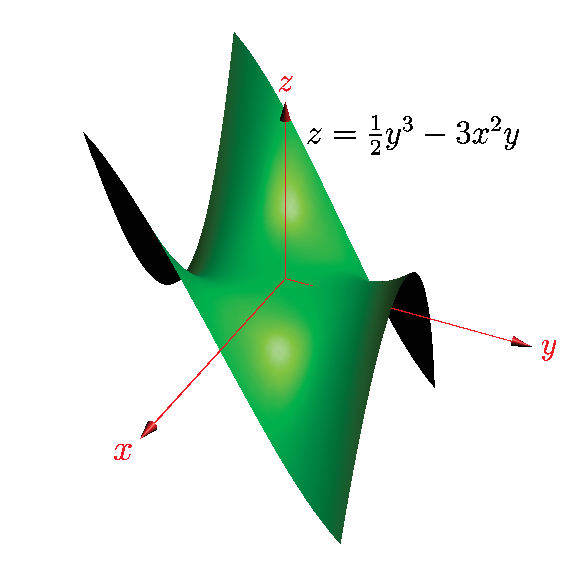
\includegraphics{mov/epixposter}}{mov/epix.prc}
%\end{frame}
%
%%\begin{frame}\titreslide{Insertion d'une image3D}
%%\includemedia[
%%label=malte,
%%width=0.5\linewidth,height=0.5\linewidth,
%%activate=pageopen,
%%3Dmenu,
%%3Dc2c=1 1 1,
%%3Dcoo=-0.001042630523443222 1.4577869224116568e-19 0.028235001489520073,
%%3Droo=0.2604540212188131,
%%add3Djscript=mov/malte.js
%%]{}{mov/malte.u3d}
%%\mediabutton[
%%jsaction=malte:{annotRM[’malte’].context3D.cntrClockWise();}
%%]{
\includegraphics[height=1.44em]{mov/boutona}}
%%\mediabutton[
%%jsaction=malte:{annotRM[’malte’].context3D.pause();}
%%]{
\includegraphics[height=1.44em]{mov/boutonb}}
%%\mediabutton[
%%jsaction=malte:{annotRM[’malte’].context3D.clockWise();}
%%]{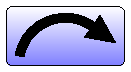
\includegraphics[height=1.44em]{mov/boutonc}}
%%\hspace{1em}
%%\mediabutton[
%%jsaction=malte:{annotRM[’malte’].context3D.scaleSpeed(1/1.1);}
%%]{
\includegraphics[height=1.44em]{mov/boutond}}
%%\mediabutton[
%%jsaction=malte:{annotRM[’malte’].context3D.origSpeed();}
%%]{
\includegraphics[height=1.44em]{mov/boutone}}
%%\mediabutton[
%%jsaction=malte:{annotRM[’malte’].context3D.scaleSpeed(1.1);}
%%]{
\includegraphics[height=1.44em]{mov/boutonf}}
%%\end{frame}
%
%\begin{frame}\titreslide{Vidéo youtube}
%\includemedia[
%  width=0.6\linewidth, height=0.45\linewidth,
%  activate=pageopen,
%  deactivate=onclick,
%  flashvars={modestbranding=1 % no YT logo in control bar
%   &autohide=1       % controlbar autohide
%   &showinfo=0       % no title and other info before start
%   &rel=0            % no related videos after end
%  }
%]{}{http://www.youtube.com/v/E0ZnwLHpZqY?rel=0}
%\end{frame}
%\subsection{Insertion d'une vidéo Youtube}
%\begin{frame}\titreslide{Insertion d'une vidéo Youtube}
%\begin{figure}
%	\begin{center}
%\includemedia[
%  width=0.6\linewidth, height=0.45\linewidth,
%  activate=pageopen,
%  deactivate=onclick,
%  flashvars={
%    modestbranding=1 % no YT logo in control bar
%   &autohide=1       % controlbar autohide
%   &showinfo=0       % no title and other info before start
%   &rel=0            % no related videos after end
%  }
%]{}{http://www.youtube.com/v/LdNu113Ep2U?rel=0}
%	\end{center}
%\end{figure}
%\end{frame}
%
%
%\begin{frame}[fragile]\titreslide{Insertion d'une animation flash}
%Il faut installer le package \verb+media9+ disponible ici : \url{http://www.ctan.org/tex-archive/macros/latex/contrib/media9} et suivre la procédure dans media9.sty. Il peut être utile de réinstaller les packages \verb+l3kernel+ and \verb+l3packages+ en utilisant \verb+Miktex Package Manager+ en mode administrateur.
%\end{frame}
%
%

\subsection{Boîtes}
\subsubsection{Boîte exemple}
\begin{frame}\titreslide{Boîte exemple}
\begin{exemple}{\null}
Ceci est un exemple
\end{exemple}

\uncover<2,3>{\begin{exemple}{autre exemple}
Ceci est un autre exemple...
\uncover<3>{\correction{Ceci est la correction}}
\end{exemple}}
\end{frame}

\subsubsection{Boîte important}
\begin{frame}\titreslide{Boîte important}
\begin{important}{\null}
toto
\end{important}
\end{frame}

\subsubsection{Boîte définition}
\begin{frame}\titreslide{Boîte définition}
\begin{madefinition}{titre}
Sujet 1:\\
Réponse 2 : \trouer{la réponse}
\end{madefinition}
\end{frame}

\begin{frame}\titreslide{Boîte définition}
\begin{madefinition}{titre2}
Sujet 1:\\
Réponse 2 : \trouer{la réponse}
\end{madefinition}
\end{frame}
%test couleur
\subsubsection{Boîte principe}
\begin{frame}\titreslide{Boîte principe}
\begin{monprincipe}{titre}
Sujet - \uncover<2>{\correction{tata}}\\
\end{monprincipe}
\end{frame}

\subsubsection{Boîte remarque}
\begin{frame}\titreslide{Boîte remarque}
\begin{remarque}{titre}
Sujet - \uncover<2>{\correction{tata}}\\
\end{remarque}
\end{frame}
\subsection{Test de boîtes}
\begin{frame}\titreslide{Teste de boîtes}
\begin{bclogo}[logo=\bcinfo,barre=none,noborder=true]{Important}%
\begin{gbar}{red}
Du texte qui se répète encore et encore pour l’exemple , du
texte qui se répète encore et encore pour l’ exemple , du texte
qui se répète encore et encore pour l’ exemple\ dots Du texte
qui se répète encore et encore pour l’ exemple , du texte qui se
répète encore et encore pour l’exemple , du texte qui se
répète encore et encore pour l’ exemple\dots
\end{gbar}
\end{bclogo}
\end{frame}

\section{Notations mathématiques}
\begin{frame}[fragile,allowframebreaks]\titreslide{Notations mathématiques}
\textbf{Symbole torseur :}\\
\SymboleTorseur

\textbf{Torseur :}\\
\Torseur{A} \Torseur{B}

\textbf{Torseur en colonne :}\\
\TorseurColonne{R}{A\\B\\C}{D\\E\\F}{A}\newline
\verb$\TorseurColonne{R}{A\\B\\C}{D\\E\\F}{A}$

\textbf{Torseur en ligne :}\\
\TorseurLigne{Point_application}{Ligne_haut}{Ligne_bas}\newline
\verb$\TorseurLigne{Point_application}{Ligne_haut}{Ligne_bas}$

\textbf{Vecteur en colonne :}\\
\VecteurColonne{repère}{A}{B}{C}\newline
\verb$\VecteurColonne{repère}{A}{B}{C}\newline$

\textbf{Vecteur}\\
\Vecteur{A}\newline
\verb$\Vecteur{A}$

\textbf{TorseurActionsMeca}\\
\TorseurActionsMeca{Fext}{S1}\newline
\verb$\TorseurActionsMeca{Fext}{S1}$

\textbf{DeriveeVecteur}\\

\textbf{Solide}
Le solide \solide{1} représente

\textbf{Paramétrage angulaire}\newline
\ParametrageAngulaire{\theta}{\vx{0}}{\vy{0}}{\vz{0}}{\vx{1}}{\vy{1}}[\vz{1}]\\

\textbf{Vitesse}\newline
\Vitesse{A}{S_1}{R_0} ou \Vitesse{A}{1}{0}\\

\Vitesseabsolue{A}{R_0}\\

\textbf{Vecteur vitesse}\newline
\VecteurVitesse{A}{S_1}{R_0} ou \VecteurVitesse{A}{1}{0}\\

\VecteurVitesseabsolue{A}{R_0}\\


\textbf{Accélération}\newline
\Acceleration{A}{S_1}{R_0} ou \Acceleration{A}{1}{0}
\Accelerationabsolue{A}{R_0}\\

\textbf{Vecteur accélération}\newline
\VecteurAcceleration{A}{S_1}{R_0} ou \VecteurAcceleration{A}{1}{0}
\VecteurAccelerationabsolue{A}{R_0}\\


\textbf{Vecteur rotation}\newline
\VecteurRotation{1}{0}

\textbf{Changement de point d'un solide}\newline
\DeplacementVitesse{1}{0}{A}{B}\\
\DeplacementVitesse{1}{0}{F}{G}

\textbf{Dérivée d'un vecteur}\newline
\DeriveeVecteur{u}{0}\\

$\DeriveeVecteur{u}{0}=\DeriveeVecteur{u}{1}+\VecteurRotation{1}{0}\vectoriel \Vecteur{u}$\\

\FormuledeBour{u}{0}{1}\\


\VecteurAcceleration{A}{1}{0}=\FormuledeBour{\Vitesse{A}{1}{0}}{0}{1}

\end{frame}
%
%\section{Insérer du code}
%\subsection{Code C++}
%\begin{frame}[fragile]\titreslide{Code C++}
%
%
%\end{frame}
%\section{Conclusion}
%test couleur

%\begin{frame}[allowframebreaks]\titreslide{Références}			
%\bibliographystyle{amsalpha}
%\bibliography{D:/Dropbox/enseignement/CPGE/raphaelpoiree/paquets/biblio}
%\end{frame}

\end{document}